\chapter{Mengenal Kecerdasan Buatan dan Scikit-Learn}
Buku umum yang digunakan adalah \cite{russell2016artificial} dan  
untuk sebelum UTS menggunakan buku \textit{Python Artificial Intelligence Projects for Beginners}\cite{eckroth2018python}.
Dengan praktek menggunakan python 3 dan editor anaconda dan library python scikit-learn.
Tujuan pembelajaran pada pertemuan pertama antara lain:
\begin{enumerate}
\item
Mengerti definisi kecerdasan buatan, sejarah kecerdasan buatan, perkembangan dan penggunaan di perusahaan
\item
Memahami cara instalasi dan pemakaian sci-kit learn
\item
Memahami cara penggunaan variabel explorer di spyder
\end{enumerate}
Tugas dengan cara dikumpulkan dengan pull request ke github dengan menggunakan latex pada repo yang dibuat oleh asisten riset.

\section{Teori}
Praktek teori penunjang yang dikerjakan :
\begin{enumerate}
\item
Buat Resume Definisi, Sejarah dan perkembangan Kecerdasan Buatan, dengan bahasa yang mudah dipahami dan dimengerti. Buatan sendiri bebas plagiat[hari ke 1](10)
\item
Buat Resume mengenai definisi supervised learning, klasifikasi, regresi dan unsupervised learning. Data set, training set dan testing set.[hari ke 1](10)
\end{enumerate}

\section{Instalasi}
Membuka https://scikit-learn.org/stable/tutorial/basic/tutorial.html. Dengan menggunakan bahasa yang mudah dimengerti dan bebas plagiat. 
Dan wajib skrinsut dari komputer sendiri.
\begin{enumerate}
\item
Instalasi library scikit dari anaconda, mencoba kompilasi dan uji coba ambil contoh kode dan lihat variabel explorer[hari ke 1](10)
\item
Mencoba Loading an example dataset, menjelaskan maksud dari tulisan tersebut dan mengartikan per baris[hari ke 1](10)
\item
Mencoba Learning and predicting, menjelaskan maksud dari tulisan tersebut dan mengartikan per baris[hari ke 2](10)
\item
mencoba Model persistence, menjelaskan maksud dari tulisan tersebut dan mengartikan per baris[hari ke 2](10)
\item 
Mencoba Conventions, menjelaskan maksud dari tulisan tersebut dan mengartikan per baris[hari ke 2](10)
\end{enumerate}


\section{Penanganan Error}
Dari percobaan yang dilakukan di atas, apabila mendapatkan error maka:

\begin{enumerate}
	\item
	skrinsut error[hari ke 2](10)
	\item
Tuliskan kode eror dan jenis errornya [hari ke 2](10)
	\item
Solusi pemecahan masalah error tersebut[hari ke 2](10)

\end{enumerate}

\section{Ahmad Syafrizal Huda/1164062}
\subsection{Teori}
\begin{enumerate}
\item Definisi, sejarah, dan perkembangan kecerdasan buatan.
\subitem Definisi kecerdasan buatan adalah suatu pengetahuan yang dapat membuat komputer untuk meniru kecerdasan manusia yang berhubungan dengan penangkapan, pemodelan, dan penyimpanan kecerdasan manusia dalam sebuah sistem teknologi. Contohnya yaitu melakukan analisa penalaran untuk mengambil suatu kesimpulan atau penerjemahan atau keputusan dari satu bahasa satu ke bahasa lain.
\subitem Sejarah dan perkembangan kecerdasan buatan terjadi pada musim panas tahun 1956 tercatat adanya seminar mengenai AI di Darmouth College. Seminar pada waktu itu dihadiri oleh sejumlah pakar komputer dan membahas potensi komputer dalam meniru kepandaian manusia. Akan tetapi perkembangan yang sering terjadi semenjak diciptakannya LISP, yaitu bahasa kecerdasan buatan yang dibuat tahun 1960 oleh John McCarthy. Istilah pada kecerdasan buatan atau Artificial Intelligence diambil dari Marvin Minsky dari MIT. Dia menulis karya ilmiah berjudul Step towards Artificial Intelligence, The Institute of radio Engineers Proceedings 49, January 1961\cite{baraja2008kecerdasan}. 
\item  Definisi supervised learning, klasifikasi, regresi, dan unsupervised learning. Data set, training set dan testing set. 
\subitem Supervised learning merupakan sebuah pendekatan dimana sudah terdapat data yang dilatih, dan terdapat variable yang ditargetkan sehingga tujuan dari pendekatan ini adalah mengkelompokan suatu data ke data yang sudah ada. Sedangkan unsupervised learning tidak memiliki data latih, sehingga dari data yang ada, kita mengelompokan data tersebut menjadi 2 bagian atau 3 bagian dan seterusnya.
\subitem Klasifikasi adalah salah satu topik utama dalam data mining atau machine learning. Klasifikasi yaitu suatu pengelompokan data dimana data yang digunakan tersebut mempunyai kelas label atau target.
\subitem Regresi adalah Supervised learning tidak hanya mempelajari classifier, tetapi juga mempelajari fungsi yang dapat memprediksi suatu nilai numerik. Contoh, ketika diberi foto seseorang, kita ingin memprediksi umur, tinggi, dan berat orang yang ada pada foto tersebut.
\subitem Data set adalah cabang aplikasi dari Artificial Intelligence/Kecerdasan Buatan yang fokus pada pengembangan sebuah sistem yang mampu belajar sendiri tanpa harus berulang kali di program oleh manusia.
\subitem Training set yaitu jika pasangan objek, dan kelas yang menunjuk pada objek tersebut adalah suatu contoh yang telah diberi label akan menghasilkan suatu algoritma pembelajaran.
\subitem Testing set digunakan untuk mengukur sejauh mana classifier berhasil melakukan klasifikasi dengan benar\cite{zhu2009introduction}.
\end{enumerate}
\subsection{Instalasi}
\subsubsection{Instalasi Library Scikit dari Anaconda}
\begin{enumerate}
\item Download aplikasi Anaconda terlebih dahulu.
\begin{figure}[ht]\centerline{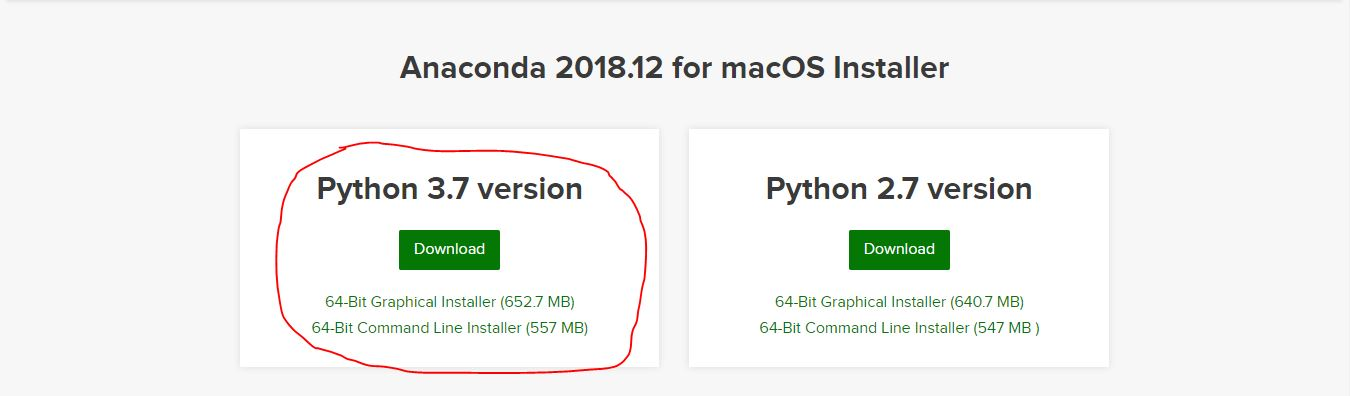
\includegraphics[width=1\textwidth]{figures/1.JPG}}\caption{Download Anaconda.}\end{figure}
\item Install aplikasi Anaconda yang sudah di download tadi.
\begin{figure}[ht]\centerline{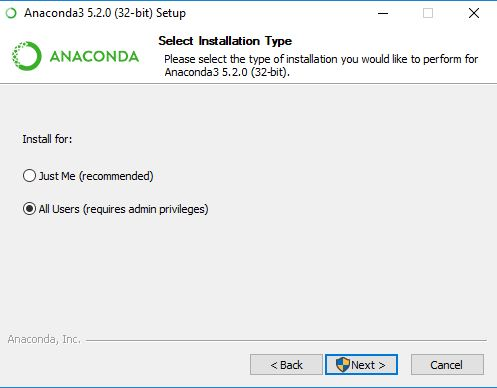
\includegraphics[width=0.75\textwidth]{figures/2.JPG}}\caption{Langkah pertama instalasi anaconda.}\end{figure}
\item Simpan aplikasi sesuai folder yang kita pilih lalu next.
\begin{figure}[ht]\centerline{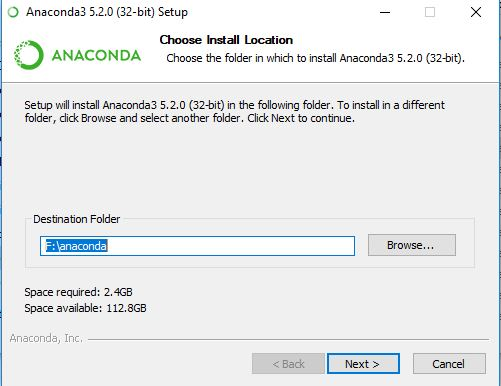
\includegraphics[width=0.75\textwidth]{figures/3.JPG}}\caption{Langkah kedua instalasi anaconda.}\end{figure}
\item Centang Keduanya lalu tekan tombol install.
\begin{figure}[ht]\centerline{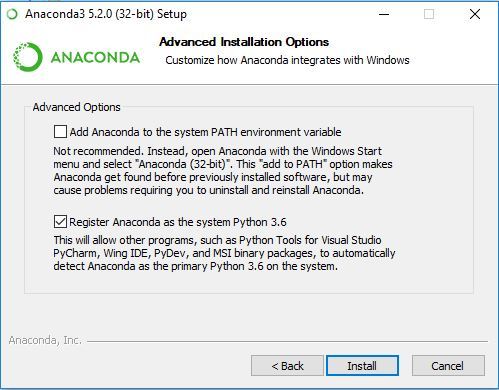
\includegraphics[width=0.75\textwidth]{figures/4.JPG}}\caption{Langkah ketiga instalasi anaconda.}\end{figure}
\item Setelah itu tunggu sampai proses instalasi selesai lalu jika sudah tekan tombol finish.
\begin{figure}[ht]\centerline{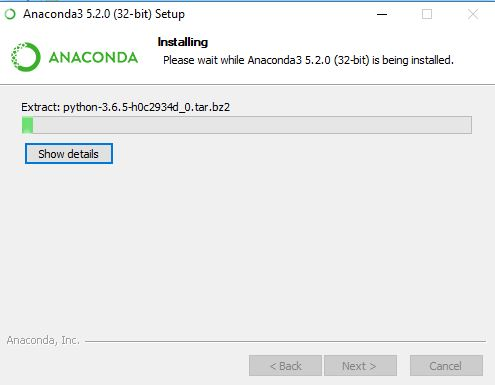
\includegraphics[width=0.75\textwidth]{figures/5.JPG}}\caption{Langkah terakhir instalasi anaconda.}\end{figure}
\item Lalu buka command prompt anda dan tuliskan perintah berikut ini untuk mengecek apakah aplikasinya sudah terinstall.
\begin{figure}[ht]\centerline{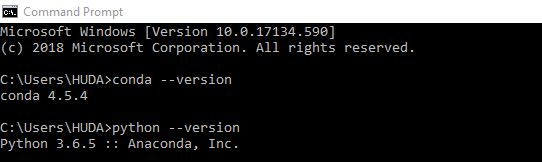
\includegraphics[width=0.75\textwidth]{figures/6.JPG}}\caption{Langkah pertama instalasi scikit pada CMD.}\end{figure}
\item Kemudian ketikkan perinta pip install -U scikit-learn seperti gambar berikut.
\begin{figure}[ht]\centerline{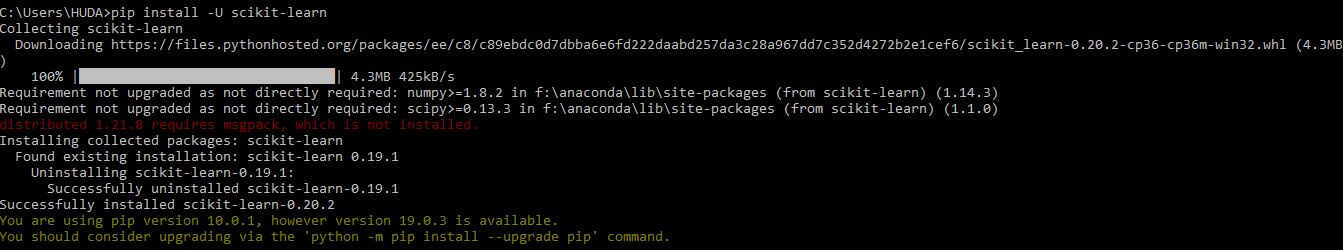
\includegraphics[width=0.75\textwidth]{figures/7.JPG}}\caption{Langkah kedua instalasi scikit pada CMD.}\end{figure}
\item Lalujika sudah  ketikkan juga perintah conda install scikit-learn.
\begin{figure}[ht]\centerline{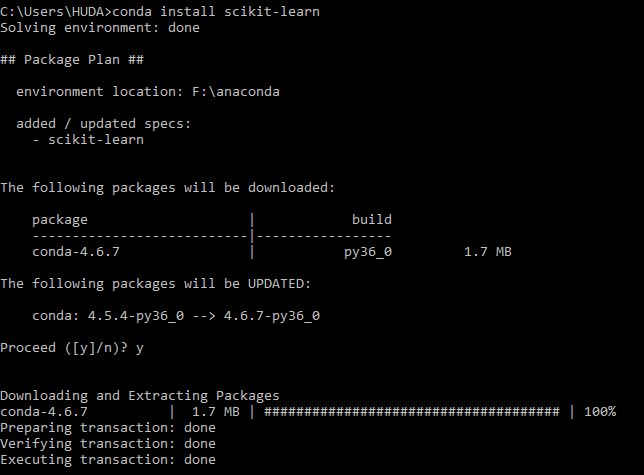
\includegraphics[width=0.75\textwidth]{figures/8.JPG}}\caption{Langkah ketiga instalasi scikit pada CMD.}\end{figure}
\item Hasil compile dari beberapa code yang mempunyai variable explorer.
\begin{figure}[ht]\centerline{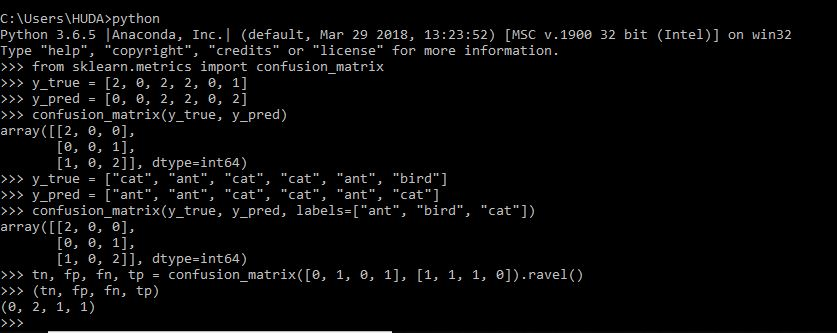
\includegraphics[width=0.75\textwidth]{figures/9.JPG}}\caption{Langkah compile code pada python anaconda.}\end{figure}
\end{enumerate}
